%LTeX: language=pt-br
% !TeX root = Apostila_IM381.tex

\cleardoublepage
\section{Elemento de barra}
\label{sec:elemento_barra}
    Na seção anterior, definimos os procedimentos para partirmos da equação diferencial do problema para chegarmos a um sistema linear que resulta numa solução aproximada para o problema. Nesta seção, definiremos as características que caracterizam o método dos elementos finitos. Mostraremos como sistematizar o procedimento da seção anterior.

    \subsection{Funções de forma definidas por trecho}

        Como um método numérico, a força do Método dos Elementos Finitos (MEF) está em sua aplicabilidade mesmo em problemas de alta complexidade geométrica. Mesmo componentes com geometrias bastante irregulares podem ter seu movimento descrito pelo MEF. Para tanto, é necessário sistematizar como definir as funções de forma que aproximam a solução.

        Não é fácil (e muitas vezes não é possível), definir um conjunto de funções no domínio de análise que obedeçam as condições de contorno de Dirichlet e que sejam linearmente independentes. Desta forma, o mais simples é subdividir esse domínio, e definir as funções apenas dentro de cada subdomínio. Cada subdomínio desses é chamado \textbf{elemento}. Ao conjunto de todos os elementos, damos o nome de \textbf{malha}.

        Desta forma, subdividimos o domínio de análise em elementos, isto é, discretizamos o domínio de análise em uma malha de elementos finitos (Figura \ref{fig:discretizacao}). Este procedimento de discretização por si só já pode gerar erros, visto que estamos aproximando as superfícies da estrutura. As funções de forma são definidas tais que cada uma delas apenas assume valores diferentes de zero em um único elemento. Considere o domínio da Figura \ref{fig:malha_barra} para a solução do problema da barra. Dividimos este domínio em quatro elementos. As funções de forma mais usuais são a ``função chapéu'', que recebe este nome devido a sua forma (Figura \ref{fig:malha_barra_forma}). Os pontos de interface entre cada elemento são chamados \textbf{nós}.

        \begin{figure}[h!]
            \centering
            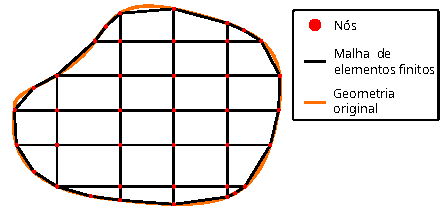
\includegraphics[scale=1]{Figures/4-Elemento_barra/Malha.pdf}
            \caption{Discretização em elementos finitos quadrangulares de uma geometria.}
            \label{fig:discretizacao}
        \end{figure}


        \begin{figure}[h!]
            \centering
            \begin{subfigure}{0.99\textwidth}
                \centering
                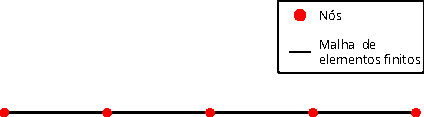
\includegraphics[scale=1]{Figures/4-Elemento_barra/Malha_Barra.pdf}
                \caption{}
                \label{fig:malha_barra}
            \end{subfigure}
            \\
            \begin{subfigure}{0.99\textwidth}
                \centering
                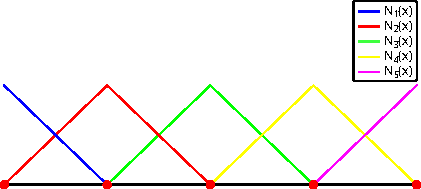
\includegraphics[scale=1]{Figures/4-Elemento_barra/Barra_Funcao_Forma.pdf}
                \caption{}
                \label{fig:malha_barra_forma}
            \end{subfigure}
            \caption{Discretização da barra. (a) Elementos e nós de um sistema de elementos de barra, (b) funções de forma ``chapéu''.}
            \label{fig:malha_barra_tot}
        \end{figure}

        Matematicamente, uma função chapéu qualquer pode ser descrita como:

        \begin{equation}
            N_i(x) = 
            \left\{
            \begin{array}{cl}
                \frac{x-x_{i-1}}{h_{i-1}} & x_{i-1} \leq x \leq x_i\\
                \frac{x_{i+1}-x}{h_i} & x_i \leq x \leq x_{i+1}\\
                0 & \text{qualquer outro ponto}\\
            \end{array}
            \right.
        \end{equation}

        \noindent no qual $h_i = x_{i+1}-x_i$ e $h_{i-1} = x_i -x_{i-1}$.

        Conforme vimos na seção anterior, precisaremos também da derivada dessa função:

        \begin{equation}
            \frac{dN_i}{dx} = 
            \left\{
            \begin{array}{cl}
                \frac{1}{h_{i-1}} & x_{i-1} \leq x \leq x_i\\
                \frac{-1}{h_i} & x_i \leq x \leq x_{i+1}\\
                0 & \text{qualquer outro ponto}\\
            \end{array}
            \right.
        \end{equation}

        Desta forma, conseguimos encontrar a matriz de rigidez do sistema resolvendo a integral:

        \begin{equation}
            \mathbf{K} = \int_0^L EA 
            \begin{Bmatrix}
            \frac{dN_1}{dx}\\
            \frac{dN_2}{dx}\\
            \vdots\\
            \frac{dN_n}{dx}\\
            \end{Bmatrix}
            \begin{bmatrix}
            \frac{dN_1}{dx} &
            \frac{dN_2}{dx} &
            \cdots &
            \frac{dN_n}{dx}
            \end{bmatrix} dx
            = \int_0^L \mathbf{B}^T \mathbf{D}\mathbf{B} dx
        \end{equation}

        \subsubsection*{Particularidade da função chapéu}

            O deslocamento aproximado pode ser reconstruído por:

            \begin{equation}
                u^h(x) = a_1 N_1(x) + a_2 N_2(x) + \cdots + a_n N_n(x)
            \end{equation}

            Considere agora o deslocamento em um nó $x_i$, apenas uma função chapéu terá valor diferente de zero, e este será unitário, isto é:

            \begin{equation}
                u^h(x) = a_i
            \end{equation}

            Portanto, ao usar funções de forma com esta propriedade, podemos chamar o vetor $\mathbf{a}$ de vetor de deslocamento nodais, e cada termo desse vetor representará o deslocamento de cada um dos nós.

            Entretanto, é precso se lembrar sempre que o MEF é um método para obter a solução aproximada ao longo de \textbf{todo} o domínio de análise, não apenas dos nós. Portanto, qualquer análise a ser feita em cima deste método \textbf{deve} considerar as interpolações em cada elemento.

            Outra particularidade na solução do problema de barra é a propriedade da \textbf{superconvergência} (Apêndice \ref{app:superconvergencia}). Para este problema, os deslocamentos nodais serão exatos, isto é, os coeficientes encontrados no sistema linear serão iguais aos deslocamentos da solução analítica (salvo erros numéricos). Note que, para um caso geral de elementos finitos, essa propriedade não se observa, isto é, \textbf{os deslocamentos nodais são aproximados.}

        \subsubsection*{Exemplo:}

            Considere uma barra com $L=1$ m com uma força distribuída uniforme de $4$ N/m e uma força concentrada de $10$ N na extremidade direita. A barra está apoiada na extremidade esquerda. Considere $E = 10^9$ Pa e $A = 10^{-6}$ m$^2$.

            Suas funções de forma serão:

            \begin{equation*}
            N_1(x) = 
            \left\{
            \begin{array}{cl}
                1-2x & 0 \leq x \leq 0.5\\
                0 & \text{qualquer outro ponto}\\
            \end{array}
            \right.
            \rightarrow
            \frac{dN_1}{dx} = 
            \left\{
            \begin{array}{cl}
                -2 & 0 \leq x \leq 0.5\\
                0 & \text{qualquer outro ponto}\\
            \end{array}
            \right.
        \end{equation*}

        \begin{equation*}
            N_2(x) = 
            \left\{
            \begin{array}{cl}
                2x & 0 \leq x \leq 0.5\\
                2-2x & 0.5 \leq x \leq 1\\
                0 & \text{qualquer outro ponto}\\
            \end{array}
            \right.
            \rightarrow
            \frac{dN_2}{dx} = 
            \left\{
            \begin{array}{cl}
                2 & 0 \leq x \leq 0.5\\
                -2 & 0.5 \leq x \leq 1\\
                0 & \text{qualquer outro ponto}\\
            \end{array}
            \right.
        \end{equation*}

        \begin{equation*}
            N_3(x) = 
            \left\{
            \begin{array}{cl}
                2x-1 & 0.5 \leq x \leq 1\\
                0 & \text{qualquer outro ponto}\\
            \end{array}
            \right.
            \rightarrow
            \frac{dN_3}{dx} = 
            \left\{
            \begin{array}{cl}
                2 & 0.5 \leq x \leq 1\\
                0 & \text{qualquer outro ponto}\\
            \end{array}
            \right.
        \end{equation*}

        Com isso, podemos encontrar a matriz de rigidez. Lembre-se que uma integral pode ser dividida como a soma de integrais cujos domínios de integração se somem no domínio original.

        \begin{equation*}
            \mathbf{K} = \int_0^1 EA 
            \begin{Bmatrix}
            \frac{dN_1}{dx}\\
            \frac{dN_2}{dx}\\
            \frac{dN_3}{dx}\\
            \end{Bmatrix}
            \begin{bmatrix}
            \frac{dN_1}{dx} &
            \frac{dN_2}{dx} &
            \frac{dN_3}{dx}
            \end{bmatrix} dx
        \end{equation*}

        \begin{equation*}
            \mathbf{K} = \int_0^{0.5} EA 
            \begin{Bmatrix}
            \frac{dN_1}{dx}\\
            \frac{dN_2}{dx}\\
            \frac{dN_3}{dx}\\
            \end{Bmatrix}
            \begin{bmatrix}
            \frac{dN_1}{dx} &
            \frac{dN_2}{dx} &
            \frac{dN_3}{dx}
            \end{bmatrix} dx + \int_{0.5}^{1} EA 
            \begin{Bmatrix}
            \frac{dN_1}{dx}\\
            \frac{dN_2}{dx}\\
            \frac{dN_3}{dx}\\
            \end{Bmatrix}
            \begin{bmatrix}
            \frac{dN_1}{dx} &
            \frac{dN_2}{dx} &
            \frac{dN_3}{dx}
            \end{bmatrix} dx
        \end{equation*}

        \begin{equation*}
            \mathbf{K} = \int_0^{0.5} EA 
            \begin{Bmatrix}
            -2\\
            2\\
            0\\
            \end{Bmatrix}
            \begin{bmatrix}
            -2 &
            2 &
            0
            \end{bmatrix} dx + \int_{0.5}^{1} EA 
            \begin{Bmatrix}
            0\\
            -2\\
            2\\
            \end{Bmatrix}
            \begin{bmatrix}
            0 &
            -2 &
            2
            \end{bmatrix} dx
        \end{equation*}

        \begin{equation*}
            \mathbf{K} = \int_0^{0.5} EA 
            \begin{bmatrix}
            4 & -4 & 0\\
            -4 & 4 & 0\\
            0 & 0 & 0
            \end{bmatrix} dx + 
            \int_{0.5}^{1} EA 
            \begin{bmatrix}
            0 & 0 & 0 \\
            0 & 4 & -4 \\
            0 & -4 & 4
            \end{bmatrix} dx
        \end{equation*}

        \begin{equation*}
            \mathbf{K} = 10^3 
            \begin{bmatrix}
            2 & -2 & 0\\
            -2 & 2 & 0\\
            0 & 0 & 0
            \end{bmatrix} + 
            10^3 
            \begin{bmatrix}
            0 & 0 & 0 \\
            0 & 2 & -2 \\
            0 & -2 & 2
            \end{bmatrix}
        \end{equation*}


        \begin{equation*}
            \mathbf{K} = 
            10^3\begin{bmatrix}
                2 & -2 & 0\\
                -2 & 4 & -2\\
                0 & -2 & 2
            \end{bmatrix}
        \end{equation*}

        Seguiremos de forma análoga para a força. Entretanto, a extremidade direita se encontra carregada com $F = 10$ N. Na extremidade esquerda, haverá a reação de apoio desconhecida $R_x$.

        \begin{equation*}
            \mathbf{f} = \mathbf{N}^T(1) F + \mathbf{N}^T(0) R_x + \int_0^1 \mathbf{N}^T p(x) dx
        \end{equation*}

        \begin{equation*}
            \mathbf{N}^T =
            \begin{Bmatrix}
                N_1(x) \\
                N_2(x) \\
                N_3(x)
            \end{Bmatrix}
        \end{equation*}

        \begin{equation*}
            \mathbf{f} = 
            \begin{Bmatrix}
                0 \\
                0 \\
                1
            \end{Bmatrix} F 
            + \begin{Bmatrix}
                1 \\
                0 \\
                0
            \end{Bmatrix} R_x 
            + \int_{0}^{0.5} 
            \begin{Bmatrix}
                1-2x\\
                2x \\
                0
            \end{Bmatrix} 4 dx 
            + \int_{0.5}^{1}
            \begin{Bmatrix}
                0\\
                2-2x \\
                2x-1
            \end{Bmatrix} 4 dx
        \end{equation*}

        \begin{equation*}
            \mathbf{f} = 
            \begin{Bmatrix}
                0 \\
                0 \\
                F
            \end{Bmatrix}
            + \begin{Bmatrix}
                R_x \\
                0 \\
                0
            \end{Bmatrix}
            + \left.
            \begin{Bmatrix}
                4x-4x^2\\
                4x^2 \\
                0
            \end{Bmatrix}\right|_{0}^{0.5}
            + \left.
            \begin{Bmatrix}
                0\\
                8x-4x^2 \\
                4x^2-4x
            \end{Bmatrix} \right|_{0.5}^{1}
        \end{equation*}

        \begin{equation*}
            \mathbf{f} = 
            \begin{Bmatrix}
                0 \\
                0 \\
                10
            \end{Bmatrix}
            + \begin{Bmatrix}
                R_x \\
                0 \\
                0
            \end{Bmatrix}
            +
            \begin{Bmatrix}
                1\\
                1\\
                0
            \end{Bmatrix}
            +
            \begin{Bmatrix}
                0\\
                4 \\
                0
            \end{Bmatrix}
            -
            \begin{Bmatrix}
                0\\
                3 \\
                -1
            \end{Bmatrix}
        \end{equation*}

        \begin{equation*}
            \mathbf{f} = 
            \begin{Bmatrix}
                1 + R_x\\
                2\\
                11
            \end{Bmatrix}
        \end{equation*}

        Portanto, o sistema linear fica da forma:

        \begin{equation*}
            \mathbf{K} \mathbf{a} = \mathbf{f} 
        \end{equation*}

        \begin{equation*}
            10^3\begin{bmatrix}
                2 & -2 & 0\\
                -2 & 4 & -2\\
                0 & -2 & 2
            \end{bmatrix}
            \begin{Bmatrix}
                a_1\\
                a_2\\
                a_3
            \end{Bmatrix}
            =
            \begin{Bmatrix}
                1 + R_x\\
                2\\
                11
            \end{Bmatrix}
        \end{equation*}

        Para aplicar as condições de contorno, usamos os procedimentos da Seção \ref{sec:condicao_contorno}, isto é, ``cortamos'' a primeira linha e a coluna do sistema (pois $a_1=0$):

        \begin{equation*}
            10^3\begin{bmatrix}
                4 & -2\\
                -2 & 2
            \end{bmatrix}
            \begin{Bmatrix}
                a_2\\
                a_3
            \end{Bmatrix}
            =
            \begin{Bmatrix}
                2\\
                11
            \end{Bmatrix}
        \end{equation*}

        Resolvendo, obtemos:

        \begin{equation*}
            a_2 = 6.5 mm
        \end{equation*}

        \begin{equation*}
            a_3 = 12 mm
        \end{equation*}

        Portanto, podemos escrever o deslocamento aproximado encontrado:

        \begin{equation*}
            u^h(x) = a_1 N_1(x) + a_2 N_2(x) + a_3 N_3(x)
        \end{equation*}

        \begin{equation*}
            u^h(x) = 
            \left\{
            \begin{array}{cl}
                13x [mm] & 0 \leq x \leq 0.5\\
                11x + 1 [mm] & 0.5 \leq x \leq 1\\
                0 & \text{qualquer outro ponto}\\
            \end{array}
            \right.
        \end{equation*}

        A solução analítica deste problema é dada por:

        \begin{equation*}
            u(x) = -2x^2 + 14 x [mm]
        \end{equation*}
 
        A Figura \ref{fig:exemplo_desl_comp} mostra uma comparação entre as soluções analítica e numérica do problema.

        \begin{figure}[h!]
            \centering
            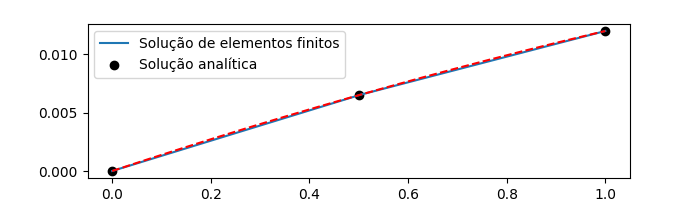
\includegraphics[scale=1]{Figures/4-Elemento_barra/Deslocamento_exemplo_4-1.png}
            \caption{Comparação entre deslocamento analítico e aproximado.}
            \label{fig:exemplo_desl_comp}
        \end{figure}

        Com a expressão do deslocamento, podemos reconstruir algumas outras grandezas associadas a ele. Por exemplo, podemos calcular a deformação aproximada em cada elemento como:

        \begin{equation*}
            \varepsilon^h(x) = \frac{du^h(x)}{dx} = a_1 \frac{d N_1}{dx} + a_2 \frac{d N_2}{dx} + a_3 \frac{d N_3}{dx} 
            = \begin{bmatrix}
            \frac{dN_1}{dx} &
            \frac{dN_2}{dx} &
            \frac{dN_3}{dx}
            \end{bmatrix}
            \begin{Bmatrix}
                a_1\\
                a_2\\
                a_3
            \end{Bmatrix}
            = \mathbf{B}\mathbf{a}
        \end{equation*}

        \begin{equation*}
            \varepsilon^h(x) = 
            \left\{
            \begin{array}{cl}
                0.013 & 0 \leq x \leq 0.5\\
                0.011 & 0.5 \leq x \leq 1\\
                0 & \text{qualquer outro ponto}\\
            \end{array}
            \right.
        \end{equation*}

        Note que, como a função chapéu é linear, a deformação então será constante dentro de cada elemento. Podemos comparar com a solução analítica (Figura \ref{fig:exemplo_def_comp}) dada por:

        \begin{figure}[h!]
            \centering
            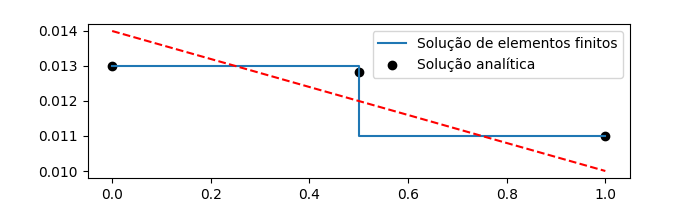
\includegraphics[scale=1]{Figures/4-Elemento_barra/Deformacao_exemplo_4-1.png}
            \caption{Comparação entre deformações analítica e aproximada.}
            \label{fig:exemplo_def_comp}
        \end{figure}

        \begin{equation*}
            \varepsilon(x) = -0.004x + 0.014
        \end{equation*}

        Podemos também comparar as tensões aproximada e analítica (Figura \ref{fig:exemplo_tens_comp}):

        \begin{figure}[h!]
            \centering
            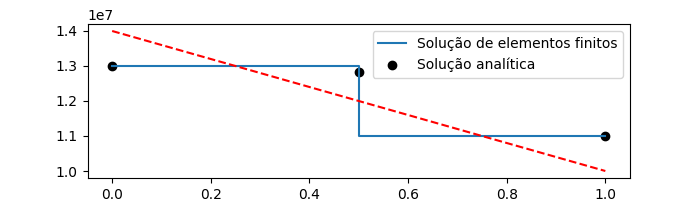
\includegraphics[scale=1]{Figures/4-Elemento_barra/Tensao_exemplo_4-1.png}
            \caption{Comparação entre tensões analítica e aproximada.}
            \label{fig:exemplo_tens_comp}
        \end{figure}

        \begin{equation*}
            \sigma^h(x) = E\varepsilon^h(x) = Ea_1 \frac{d N_1}{dx} + Ea_2 \frac{d N_2}{dx} + Ea_3 \frac{d N_3}{dx} 
            = E\begin{bmatrix}
            \frac{dN_1}{dx} &
            \frac{dN_2}{dx} &
            \frac{dN_3}{dx}
            \end{bmatrix}
            \begin{Bmatrix}
                a_1\\
                a_2\\
                a_3
            \end{Bmatrix}
            = \mathbf{D}\mathbf{B}\mathbf{a}
        \end{equation*}

        \begin{equation*}
            \sigma^h(x) = 
            \left\{
            \begin{array}{cl}
                13 MPa & 0 \leq x \leq 0.5\\
                11 MPa & 0.5 \leq x \leq 1\\
                0 & \text{qualquer outro ponto}\\
            \end{array}
            \right.
        \end{equation*}

        \begin{equation*}
            \sigma(x) = -4x + 14 [MPa]
        \end{equation*}

        Finalmente, podemos verificar a reação de apoio e o esforço normal interno na barra. Para encontrar a reação $R_x$, podemos voltar a equação que descartamos do sistema linear e resolvê-la:

        \begin{equation*}
            R_x = -14 N
        \end{equation*}

        Comparamos então os esforços internos:

        \begin{equation*}
            N_x(0) = \left.EA\frac{du}{dx}\right|_{x=0} = -4x+14 = 14 N
        \end{equation*}

        \begin{equation*}
            N_x(1) = \left.EA\frac{du}{dx}\right|_{x=1} = -4x+14 = 10 N
        \end{equation*}

        \begin{equation*}
            N_x^h(0) = \left.EA\frac{du^h}{dx}\right|_{x=0} = 13N
        \end{equation*}

        \begin{equation*}
            N_x^h(1) = \left.EA\frac{du^h}{dx}\right|_{x=1} = 11 N
        \end{equation*}

        Perceba que, embora a reação de apoio seja igual à reação analítica ($N_x(0)$), a condição de contorno de Neumann imposta não é exata, isto é $N_x^h(L) \neq N_x(L)$.

    \subsection{Matriz elementar}

        O procedimento mostrado anteriormente ainda é bastante trabalhoso. Podemos simplificá-lo, dividindo a integração elemento a elemento. Note que, ao integrarmos no exemplo, já tivemos que dividir o domínio de integração nos elementos. Portanto, podemos já fazer isso logo de início, integrar uma matriz menor para cada elemento, e depois juntá-la numa matriz maior.

        Considere o $e$-ésimo elemento de uma malha de elementos de barra, ele terá as seguintes funções de forma dentro dele:

        \begin{equation}
            N_1(x) = \frac{x_{e+1}-x}{h_e} \rightarrow \frac{dN_1}{dx} = -\frac{1}{h_e}
        \end{equation}

        \begin{equation}
            N_2(x) = \frac{x-x_e}{h_e} \rightarrow \frac{dN_2}{dx} = \frac{1}{h_e}
        \end{equation}

        Uma integração no domínio total da estrutura $\Omega$ pode ser subdividido na soma de integrais no domínio de cada elemento da malha (Figura \ref{fig:dominio_discretizado}):

        \begin{equation}
            \int_{\Omega} f(x) dA = \int_{\Omega_{e_1}} f(x) dA + \int_{\Omega_{e_2}} f(x) dA + \cdots + \int_{\Omega_{e_n}} f(x) dA
        \end{equation}

        \begin{figure}[h!]
            \centering
            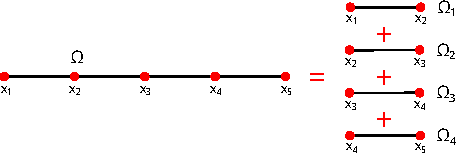
\includegraphics[scale=1.3]{Figures/4-Elemento_barra/Dominio.pdf}
            \caption{Dividindo o intervalo de integração nos vários elementos}
            \label{fig:dominio_discretizado}
        \end{figure}

        Portanto, em vez de montar a matriz do sistema global de uma vez, podemos encontrar uma matriz para cada elemento, avaliando a integral no domínio deste elemento.

        Considerando um elemento de barra $e$:

        

        \begin{equation*}
            \mathbf{K}_e = \int_{x_e}^{x_{e+1}} \mathbf{B}_e^T \mathbf{D}_e\mathbf{B}_e dx = \int_{x_e}^{x_{e+1}} EA 
            \begin{Bmatrix}
            \frac{dN_1}{dx}\\
            \frac{dN_2}{dx}
            \end{Bmatrix}
            \begin{bmatrix}
            \frac{dN_1}{dx} &
            \frac{dN_2}{dx}
            \end{bmatrix} dx
        \end{equation*}

        \begin{equation*}
            \mathbf{K}_e = \int_{x_e}^{x_{e+1}} EA 
            \begin{Bmatrix}
            -\frac{1}{h_e}\\
            \frac{1}{h_e}
            \end{Bmatrix}
            \begin{bmatrix}
            -\frac{1}{h_e} &
            \frac{1}{h_e}
            \end{bmatrix} dx
        \end{equation*}

        \begin{equation*}
            \mathbf{K}_e = \int_{x_e}^{x_{e+1}} \frac{EA}{h_e^2} 
            \begin{Bmatrix}
            -1\\
            1
            \end{Bmatrix}
            \begin{bmatrix}
            -1 &
            1
            \end{bmatrix} dx
        \end{equation*}

        \begin{equation*}
            \mathbf{K}_e = 
            \frac{EA}{h_e^2}\begin{bmatrix}
                1 & -1\\
                -1 & 1
            \end{bmatrix}
            \int_{x_e}^{x_{e+1}} dx
        \end{equation*}

        \begin{equation*}
            \mathbf{K}_e = 
            \frac{EA}{h_e^2}\begin{bmatrix}
                1 & -1\\
                -1 & 1
            \end{bmatrix}
            \left(x_{e+1} - x_e\right)
        \end{equation*}


        \begin{equation}
            \mathbf{K}_e = 
            \frac{EA}{h_e}\begin{bmatrix}
                1 & -1\\
                -1 & 1
            \end{bmatrix}
        \end{equation}

        Similarmente, podemos avaliar a integral da força elemento a elemento. Considere o mesmo elemento de barra com uma força distribuída uniforme $p$.


        \begin{equation*}
            \mathbf{f}_e = \int_{x_e}^{x_{e+1}} 
            \begin{Bmatrix}
            N_1\\
            N_2
            \end{Bmatrix} 
            p dx =
            \int_{x_e}^{x_{e+1}} 
            \begin{Bmatrix}
            \frac{x_{e+1}-x}{h_e}\\
            \frac{x-x_e}{h_e}
            \end{Bmatrix} 
            p dx
        \end{equation*}

        \begin{equation*}
            \mathbf{f}_e = 
            \left. p
            \begin{Bmatrix}
            \frac{2x_{e+1}x-x^2}{2h_e}\\
            \frac{x^2-2x_e x}{2h_e}
            \end{Bmatrix}\right|_{x_e}^{x_{e+1}} =
            p
            \begin{Bmatrix}
            \frac{x_{e+1}^2-2x_{e+1}x_e+x_e^2}{2h_e}\\
            \frac{x_{e+1}^2-2x_{e+1}x_e+x_e^2}{2h_e}
            \end{Bmatrix} = 
            p
            \begin{Bmatrix}
            \frac{\left(x_{e+1}-x_e\right)^2}{2h_e}\\
            \frac{\left(x_{e+1}-x_e\right)^2}{2h_e}
            \end{Bmatrix}
        \end{equation*}

        \begin{equation*}
            \mathbf{f}_e = 
            p
            \begin{Bmatrix}
            \frac{h_e^2}{2h_e}\\
            \frac{h_e^2}{2h_e}
            \end{Bmatrix} = 
            p
            \begin{Bmatrix}
            \frac{h_e}{2}\\
            \frac{h_e}{2}
            \end{Bmatrix}
        \end{equation*}

        \begin{equation*}
            \mathbf{f}_e = \frac{p h_e}{2}
            \begin{Bmatrix}
                1\\
                1 
            \end{Bmatrix}
        \end{equation*}


    \subsection{Montagem do sistema global}

        Um dado elemento $e$ vai ter sua matriz de rigidez $\mathbf{K}_e$ e seu vetor de forças $\mathbf{f}_e$. Este elemento apenas contém uma parte de todas as funções de forma do sistema (no caso da barra, duas), e portanto, essa matriz e esse vetor serão de tamanho bastante inferior ao tamanho da matriz global.

        Considerando o mesmo elemento anterior, o sistema deste elemento, fica $2 \times 2$, da seguinte forma:

        \begin{equation}
            \mathbf{K}_e \mathbf{a}_e = \mathbf{f}_e 
        \end{equation}
        
        \begin{equation}
            \frac{EA}{h_e}\begin{bmatrix}
                1 & -1\\
                -1 & 1
            \end{bmatrix}
            \begin{Bmatrix}
                a_{e}\\
                a_{e+1}\\
            \end{Bmatrix}=
            \begin{Bmatrix}
                f_{e}\\
                f_{e+1}\\
            \end{Bmatrix}
        \end{equation}

        Talvez uma das primeiras coisas que o leitor possa perceber é que o sistema acima não possui solução única. Isso é esperado, visto que um elemento é apenas uma pequena parte do sistema completo e por si só não representa adequadamente o sistema.

        O sistema global, conforme mostrado anteriormente, incluirá todos os graus de liberdade do sistema, inclusive aqueles apenas presentes em outros elementos:

        \begin{equation}
            \begin{bmatrix}
                K_{11} & K_{12} & \cdots & K_{1n}\\
                K_{21} & K_{22} & \cdots & K_{2n}\\
                \vdots & \vdots & \ddots & \vdots\\
                K_{n1} & K_{n2} & \cdots & K_{nn}\\
            \end{bmatrix}
            \begin{Bmatrix}
                a_1\\
                a_2\\
                \vdots\\
                a_n
            \end{Bmatrix}
            =
            \begin{Bmatrix}
                f_1\\
                f_2\\
                \vdots\\
                f_n
            \end{Bmatrix}
        \end{equation}

        Portanto, para obtermos o sistema global, precisamos fazer o procedimento de montagem da matriz de global. A montagem é feita da seguinte forma: verificamos a matriz de rigidez elementar do elemento que estamos analisando. Vemos os deslocamentos deste elemento. Inserimos os termos da matriz elementar na matriz global, nas linhas e colunas correspondentes àquele deslocamento. O procedimento de montagem muitas vezes tem a seguinte notação:

        \begin{equation}
            \mathbf{K} = \assembly_{e=1}^n \mathbf{K}_e
        \end{equation}
 

        Por exemplo, considere uma barra sujeita a uma carga distribuída uniforme, discretizada em dois elementos. O primeiro elemento possui os graus de liberdade $1$ e $2$. O segundo possui os graus de liberdade $2$ e $3$. A montagem da matriz e vetor globais, é feita inserindo esses termos nas posições correspondentes na matriz global, isto é:

        \begin{equation*}
            \mathbf{K} = 
            \begin{bmatrix}
                \frac{EA}{h_1} & -\frac{EA}{h_1} & 0\\
                -\frac{EA}{h_1} & \frac{EA}{h_1} + \frac{EA}{h_2} & -\frac{EA}{h_2}\\
                0 & -\frac{EA}{h_2} & \frac{EA}{h_2}
            \end{bmatrix}
        \end{equation*}

        \begin{equation*}
            \mathbf{f} = 
            \begin{Bmatrix}
                \frac{p h_1}{2}\\
                \frac{p h_1}{2} + \frac{p h_2}{2}\\
                \frac{p h_2}{2}
            \end{Bmatrix}
        \end{equation*}

        Portanto, em vez de resolvermos as integrais no domínio global, montamos as matrizes de rigidez de cada elemento (note que, se os elementos forem idênticos, suas matrizes serão iguais!). Montadas a matriz e vetor globais, nós realizamos o procedimento de montagem.

        Esta abordagem nos permite simplificar as integrais, reduzindo o domínio de integração de uma geometria possivelmente complexa na soma de integrais em geometrias mais simples (como quadrados e triângulos no 2D). Ela também nos permite adicionar tipos diferentes de elementos em locais diferentes do domínio.

        Nas próximas seções, veremos como tratar cada elemento. Como definir as funções de forma em coordenadas locais centradas no próprio elemento de análise, nos permitindo a construção de ``blocos'' para montar a malha, independentemente de onde esse elemento estará.

        \subsubsection*{Propriedades da matriz global}

        Antes de continuar a trabalhar nos elementos e suas funções de forma, vamos salientar algumas propriedades importantes da matriz de rigidez de elementos finitos. Em muitos casos, para simular de forma precisa alguma estrutura, precisamos usar milhões ou até bilhões de elementos finitos. Nestes casos, chegamos à matrizes com possivelmente centenas de milhões ou até bilhões de linhas e colunas. Evidentemente, se a solução de um sistema linear desta magnitude fosse impossível, o MEF não seria um método tão importante na engenharia quanto ele é. Esta seção discutirá algumas propriedades da matriz que torna esse sistema linear viável de resolver.

        A matriz de rigidez elementar (e consequentemente a global), será simétrica e semi-positivo definida. Uma matriz é dita semi-positivo definida quando:

        \begin{equation}
            x^T K x \geq 0, \quad \forall x \in \mathcal{R}^n,
        \end{equation}

        \noindent isto é equivalente a dizer que todos os autovalores da matriz são não negativos (positivos ou nulos).

        Após aplicar as condições de contorno suficientes para tornar o sistema isostático ou hiperestático, a matriz se torna positivo definida. Neste caso, seus autovalores serão estritamente positivos e a desigualdade da expressão acima tem um operador de maior, em vez de maior ou igual. A consequência direta dessa propriedade é que o sistema linear terá apenas uma solução.

        Outra vantagem dessas propriedades da matriz de rigidez está na seleção dos métodos de solução do sistema. A matriz ser simétrica e real permite a utilização da fatoração de Cholesky (similar a fatoração LU, porém com $L = U^T$, utilizando metade da memória e do tempo). A matriz ser positivo-definida permite a aplicação de métodos iterativos na solução do sistema (comuns em casos muito grandes), como o método dos Gradientes Conjugados.

        Entretanto, a propriedade mais importante dessas matrizes, é que elas são esparsas. Uma matriz esparsa é uma matriz cuja grande maioria dos termos é nula. No MEF, a matriz global terá os termos da diagonal principal não nulos. Fora da diagonal principal, serão não nulos apenas termos correspondentes a deslocamentos que compartilham algum elemento. No caso de uma malha com elementos de barra dispostos sequencialmente, cada linha da matriz terá, no máximo, três termos não nulos, mesmo que a matriz tenha milhões de linhas! Similarmente, se temos um elemento quadrado com quatro nós, cada um com deslocamento horizontal e vertical, cada linha da matriz global terá, no máximo, 18 termos não nulos. Note que, além de possuir poucos termos não nulos, o número máximo possível é bastante previsível.

        Na computação, existem duas formas de armazenar matrizes na memória. A primeira e mais usual é armazená-la como uma matriz densa. Uma matriz densa possui todos os seus elementos salvos na memória de forma explícita. Por exemplo, uma matriz 100x100, ocupará um espaço de 10 mil variáveis \textit{float} na memória. Outra forma de salvar uma matriz na memória é como uma matriz esparsa. Existem várias formas de armazenar uma matriz esparsa, mas a mais usual é salvá-la como COO (lista coordenada). Em vez de salvar cada termo, salvam-se apenas os termos não nulos (Figura \ref{fig:matriz_esparsa}). Para isso, para cada um deles, salvam-se três valores: sua linha, sua coluna e seu valor. No exemplo de uma matriz 100x100, considerando 5 termos não nulos por linha, teremos apenas 500 não nulos na matriz inteira. Portanto, precisamos de apenas 1000 variáveis do tipo \textit{int} e 500 do tipo float para armazenar a mesma matriz que necessitaria de 10 mil \textit{floats} para armazenar como densa.

        \begin{figure}[h!]
            \centering
            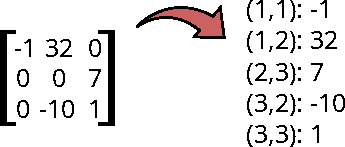
\includegraphics[scale=1]{Figures/4-Elemento_barra/Esparsa.pdf}
            \caption{Representação de uma matriz como uma matriz densa e como uma matriz esparsa do tipo COO.}
            \label{fig:matriz_esparsa}
        \end{figure}

        Por exemplo, considere um problema de MEF 2D de condução de calor com um milhão de elementos. Cada linha, neste caso, terá nove termos não nulos. O número total de linhas na matriz será por volta de um milhão também, então suponhamos que continue com este valor, para simplificar o exemplo. Se armazenássemos essa matriz de forma densa, precisariamos salvar $10^6 \times 10^6 = 10^{12}$ termos do tipo \textit{float}. Supondo que cada variável ocupe 8 \textit{bytes} na memória, precisaríamos de $73$ TB de memória! Nem um disco rígido médio seria capaz de armazenar esta matriz!

        Como uma matriz COO, considerando que as duas variáveis \textit{int} e a variável \textit{float} ocupem o mesmo espaço na memória, teremos apenas $9 \times 3 \times 10^6 = 27 \cdot 10^6$ termos para salvar. Considerando os mesmos 8 \textit{bytes} por termo, reduzimos o espaço na memória para apenas $206$ MB! Reduz-se o custo em memória para um valor que até a memória RAM de um \textit{smartwatch} ou uma calculadora gráfica seria capaz de armazenar!


    \subsection{Coordenadas locais e mudança de coordenadas}

        Na seção anterior, vimos que precisamos calcular apenas as matrizes elementares de cada elemento. Feito esse cálculo, apenas montamos eles para chegarmos na matriz global. Entretanto, a matriz elementar ainda possui limites de integração que dependem da posição do elemento na malha. Para modificar essa integração, tornando-a menos dependente diretamente da posição do elemento, utilizaremos coordenadas locais em cada elemento.

        Considere o elemento na Figura \ref{fig:coord_local_barra}. Definiremos um sistema de coordenadas locais $\xi$. Desta forma, todo elemento de barra será mapeado para este elemento em coordenadas locais. O sistema de coordenadas em coordenadas locais sempre será definido com os limites de $-1$ a $1$, para utilizarmos o procedimento de integração numérica da próxima seção. Portanto, os dois nós do elemento de barra estarão em $\xi_1 = -1$ e $\xi_2 = 1$, para cada elemento.

        \begin{figure}[h!]
            \centering
            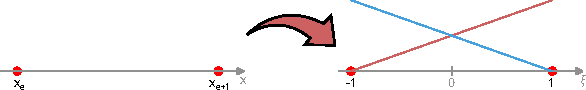
\includegraphics[scale=1.5]{Figures/4-Elemento_barra/Coordenada_local.pdf}
            \caption{Mudança de coordenadas de um elemento de barra de coordenadas globais para coordenadas locais. Funções de forma representadas na coordenada local.}
            \label{fig:coord_local_barra}
        \end{figure}

        Ademais, as funções de forma de cada elemento serão definidas em coordenadas locais. De forma similar a seção anterior, as funções de forma do elemento de barra com dois nós são:

        \begin{equation*}
            N_1(\xi) = \frac{1}{2}\left(1-\xi\right)
       \end{equation*}

       \begin{equation*}
            \frac{dN_1}{d\xi} = -\frac{1}{2}
       \end{equation*}

       \begin{equation*}
            N_2(\xi) = \frac{1}{2}\left(1+\xi\right)
       \end{equation*}

       \begin{equation*}
            \frac{dN_2}{d\xi} = \frac{1}{2}
       \end{equation*}

       Portanto, o deslocamento em um dado elemento é dado por:

       \begin{equation*}
            u^h(\xi) = N_1(\xi) a_1 + N_2(\xi) a_2
       \end{equation*}

       Se considerarmos que o elemento de barra em questão possui como nós os pontos com coordenadas $x_i$ e $x_{i+1}$, podemos definir um mapeamento entre a coordenada global $x$ e a coordenada local $\xi$ pelas funções de forma:

       \begin{equation*}
            x(\xi) = N_1(\xi) x_i + N_2(\xi) x_{i+1}
       \end{equation*}

       A derivada desse mapeamento será importante nas deduções a seguir, portanto vamos escrevê-la aqui:

       \begin{equation*}
            \frac{dx}{d\xi} = \frac{dN_1}{d\xi} x_i + \frac{dN_2}{d\xi} x_{i+1}
       \end{equation*}

       \begin{equation}
            \frac{dx}{d\xi} = \frac{x_{i+1}-x_i}{2} = \frac{h_e}{2}
       \end{equation}

       No caso unidimensional, temos essa expressão da derivada. Em casos 2D ou 3D, teremos um sistema com duas ou três coordenadas, respectivamente, tanto globais quanto locais. A combinação das derivadas das coordenadas globais em relação às locais definira um termo conhecido como \textbf{matriz Jacobiana}. O determinante dessa matriz representa a razão do comprimento/área/volume (a depender se é 1D, 2D ou 3D) entre o elemento em coordenadas globais e locais.

       Também precisaremos do inverso dessa derivada, para isso, usamos a regra da cadeia:

       \begin{equation*}
            \frac{dx}{d\xi} \frac{d\xi}{dx} = \frac{dx}{dx} = 1 
       \end{equation*}

       \begin{equation*}
            \frac{d\xi}{dx} = \left(\frac{dx}{d\xi}\right)^{-1} = \frac{2}{h_e}
       \end{equation*}

       Finalmente, para calcularmos a matriz de rigidez do elemento, precisamos dos termos $\frac{dN_1}{dx}$ e $\frac{dN_2}{dx}$. Note que as derivadas são em relação \textbf{às coordenadas globais, não às locais!} Uma grande fonte de erro é utilizar as derivadas $\frac{dN_1}{d\xi}$ em vez de $\frac{dN_1}{dx}$ na montagem da matriz. Para encontramos a derivada em relação à coordenada global, podemos usar a regra da cadeia, novamente:

       \begin{equation*}
            \frac{dN_1}{dx} = \frac{dN_1}{d\xi} \frac{d\xi}{dx} = -\frac{1}{2} \frac{2}{h_e} = -\frac{1}{h_e}
       \end{equation*}

       \begin{equation*}
            \frac{dN_2}{dx} = \frac{dN_2}{d\xi} \frac{d\xi}{dx} = \frac{1}{2} \frac{2}{h_e} = \frac{1}{h_e}
       \end{equation*}


       \begin{equation*}
            \mathbf{B} = 
            \begin{bmatrix}
            \frac{dN_1}{dx} &
            \frac{dN_2}{dx}
            \end{bmatrix} = 
            \begin{bmatrix}
            -\frac{1}{h_e} &
            \frac{1}{h_e}
            \end{bmatrix}=
            \frac{1}{h_e}
            \begin{bmatrix}
            -1 &
            1
            \end{bmatrix}
       \end{equation*}

       Finalmente, voltamos à integração da matriz elementar:

       \begin{equation*}
            \mathbf{K}_e = \int_{\Omega_e} \mathbf{B}^T \mathbf{D} \mathbf{B} dx
        \end{equation*}

        Do Cálculo, podemos nos lembrar que é possível modificar o domínio de integração por mudança de coordenadas da seguinte forma:

        \begin{equation*}
            \int_{\Omega_x} f(x) dx = \int_{\Omega_y} f(x(y)) \frac{dx}{dy} dy
        \end{equation*}


        Portanto, para o elemento de barra:

        \begin{equation*}
            \mathbf{K}_e = \int_{\Omega_e} \mathbf{B}^T \mathbf{D} \mathbf{B} dx
        \end{equation*}


        \begin{equation*}
            \mathbf{K}_e = \int_{-1}^1 \mathbf{B}^T \mathbf{D} \mathbf{B} \frac{dx}{d\xi} d\xi
        \end{equation*}


        \begin{equation*}
            \mathbf{K}_e = \int_{-1}^1 \frac{EA}{h_e^2}
            \begin{Bmatrix}
            -1 \\
            1
            \end{Bmatrix}
            \begin{bmatrix}
            -1 &
            1
            \end{bmatrix} \frac{h_e}{2} d\xi
        \end{equation*}

        \begin{equation*}
            \mathbf{K}_e =  \frac{EA}{2h_e}
            \begin{bmatrix}
             1 & -1\\
            -1 &  1
            \end{bmatrix} \int_{-1}^1 d\xi
        \end{equation*}

        \begin{equation*}
            \mathbf{K}_e = 
            \frac{EA}{h_e}
            \begin{bmatrix}
                1 & -1 \\
                -1 & 1 \\
            \end{bmatrix}
        \end{equation*}

        Chegamos ao mesmo resultado que o anterior. Embora possa parecer trivial para o caso da barra, mostraremos como isso pode simplificar ao modificar as funções de forma na seção seguinte.

        A mesma coisa pode ser feita para o vetor de forças:

        \begin{equation*}
            f_{1} = \int_{\Omega_e} N_1(x) p(x) dx = \int_{-1}^1 N_1(\xi) p(\xi) \frac{dx}{d\xi} d\xi
        \end{equation*}

        \begin{equation*}
            f_{2} = \int_{\Omega_e} N_2(x) p(x) dx = \int_{-1}^1 N_2(\xi) p(\xi) \frac{dx}{d\xi} d\xi
        \end{equation*}

    \subsection{Polinômios de Lagrange}
    \label{sec:lagrange}

        Já passamos toda a formulação do elemento em coordenadas locais, mantendo apenas o termo de transformação da variável de integração e da regra da cadeia das derivadas internas. Desta forma, temos agora a liberdade de modificar as funções de forma do elemento.

        De forma geral, as funções de forma são polinomiais. Mais especificamente, no MEF, são utilizados os polinômios de Lagrange. Os polinômios de Lagrange são um conjunto de $n+1$ polinômios de grau $n$ que interpolam $n+1$ pontos, de forma que apenas um deles é não nulo em cada ponto. Isto é, para definir um conjunto de polinômios de Lagrange de grau $n$, seguimos o procedimento:

        
        \begin{enumerate}
            \item Dados $n+1$ pontos $\left\{x_0, x_1, \cdots, x_n\right\}$;
            \item Os $n+1$ polinômios de Lagrange de ordem $n$ $\left\{l_0(x), l_1(x), \cdots, l_n(x)\right\}$ são aqueles que têm a propriedade:
            
            \begin{equation*}
                \begin{array}{cccc}
                    l_0(x_0) = 1 & l_0(x_1) = 0 & \cdots & l_0(x_n) = 0\\
                    l_1(x_0) = 0 & l_1(x_1) = 1 & \cdots & l_1(x_n) = 0\\
                    \vdots & \vdots & \ddots & \vdots\\
                    l_n(x_0) = 0 & l_n(x_1) = 0 & \cdots & l_n(x_n) = 1\\
                \end{array}
            \end{equation*}
        \end{enumerate}

        A grande consequência desta propriedade dos polinômios de Lagrange, é que, dada uma função definida pela composição desses polinômios:

        \begin{equation}
            f(x) = \sum\limits_{i=1}^{n+1} l_i(x) a_i,
        \end{equation}

        Em cada um dos pontos definidos, o valor da função será exatamente o coeficiente correspondente ao polinômio de Lagrange que é não nulo naquele ponto:

        \begin{equation}
            f(x_i) = a_i.
        \end{equation}

        Portanto, no contexto de elementos finitos, em que cada um desses pontos serão nós da malha, o deslocamento nos nós serão exatamente os termos do vetor de deslocamento nodal:

        \begin{equation}
            u(\xi_i) = \sum\limits_{i=1}^{n+1} l_i(\xi_i) a_i = a_i 
        \end{equation}

        Perceba que, até o momento, \textbf{já estamos utilizando o par de polinômios de Lagrange de grau 1!} Portanto, precisamos apenas saber como montar elementos de ordem superior, sendo a ordem do elemento definida como o grau das suas funções de forma.

        \subsubsection*{Exemplo: grau 1}

        \begin{equation*}
                \xi_0 = -1, \quad \xi_1 = 1
            \end{equation*}

        \begin{equation*}
            \begin{array}{cc}
                N_1(-1) = 1 & N_1(1) = 0\\
                N_2(-1) = 0 & N_2(1) = 1
            \end{array}
        \end{equation*}

        \begin{equation*}
            N_1(\xi) = a_0 + b_0 \xi
        \end{equation*}

        \begin{equation*}
            1 = a_0 - b_0, \quad 0 = a_0 + b_0
        \end{equation*}

        \begin{equation*}
            a_0 = \frac{1}{2}, \quad b_0 = -\frac{1}{2}
        \end{equation*}

        \begin{equation*}
            N_1(\xi) = \frac{1}{2}\left(1-\xi\right)
        \end{equation*}

        \begin{equation*}
            N_2(\xi) = \frac{1}{2}\left(1+\xi\right)
        \end{equation*}

        \subsubsection*{Exemplo: grau 2}

        \begin{equation*}
                \xi_0 = -1, \quad \xi_1 = 0 , \quad \xi_2 = 1
            \end{equation*}

        \begin{equation*}
            \begin{array}{ccc}
                N_1(-1) = 1 & N_1(0) = 0 & N_1(1) = 0\\
                N_2(-1) = 0 & N_2(0) = 1 & N_2(1) = 0\\
                N_3(-1) = 0 & N_3(0) = 0 & N_3(1) = 1\\
            \end{array}
        \end{equation*}

        \begin{equation*}
            N_1(\xi) = a_0 + b_0 \xi + c_0 \xi^2
        \end{equation*}

        \begin{equation*}
            1 = a_0 - b_0 + c_0, \quad 0 = a_0 , \quad 0 = a_0 + b_0 + c_0
        \end{equation*}

        \begin{equation*}
            a_0 = 0, \quad b_0 = -\frac{1}{2} , \quad c_0 = \frac{1}{2}
        \end{equation*}

        \begin{equation*}
            N_1(\xi) = \frac{\xi}{2}\left(\xi-1\right) \rightarrow \frac{dN_1}{d\xi} = \xi-\frac{1}{2}
        \end{equation*}

        \begin{equation*}
            N_2(\xi) = 1-\xi^2 \rightarrow \frac{dN_2}{d\xi} = -2\xi
        \end{equation*}

        \begin{equation*}
            N_3(\xi) = \frac{\xi}{2}\left(\xi+1\right) \rightarrow \frac{dN_3}{d\xi} = \xi+\frac{1}{2}
        \end{equation*}

        \begin{equation*}
            x(\xi) = N_1(\xi) x_i + N_2(\xi) x_{i+1} + N_3(\xi) x_{i+2}
        \end{equation*}

       \begin{equation*}
            \frac{dx}{d\xi} = \frac{dN_1}{d\xi} x_i + \frac{dN_2}{d\xi} x_{i+1} + \frac{dN_3}{d\xi} x_{i+2}
       \end{equation*}

       \begin{equation*}
            \frac{dx}{d\xi} = \left(\xi-\frac{1}{2}\right) x_i - 2\xi x_{i+1} + \left(\xi+\frac{1}{2}\right) x_{i+2}
       \end{equation*}

       \begin{equation*}
            \frac{dx}{d\xi} = \xi \left(x_i - 2x_{i+1} + x_{i+2}\right) + \frac{x_{i+2}-x_i}{2}
       \end{equation*}

       Se considerarmos que $x_{i+1}$ está no meio dos outros dois pontos $\left(x_{i+1} = \frac{x_{i+2}+x_i}{2}\right)$:

       \begin{equation*}
            \frac{dx}{d\xi} =\frac{h_e}{2}
       \end{equation*}

       \begin{equation*}
            \frac{d\xi}{dx} =\frac{2}{h_e}
       \end{equation*}

       \begin{equation*}
            \frac{dN_1}{dx} = \frac{dN_1}{d\xi} \frac{d\xi}{dx}  = \frac{1}{h_e}\left(2\xi-1\right)
        \end{equation*}

        \begin{equation*}
            \frac{dN_2}{dx} = \frac{dN_2}{d\xi} \frac{d\xi}{dx} = -\frac{4\xi}{h_e}
        \end{equation*}

        \begin{equation*}
            \frac{dN_3}{dx} = \frac{dN_3}{d\xi} \frac{d\xi}{dx} = \frac{1}{h_e}\left(2\xi+1\right)
        \end{equation*}

        \begin{equation*}
            \mathbf{K}_e = \int_{-1}^{1} \mathbf{B}^T\mathbf{D}\mathbf{B} \frac{dx}{d\xi} d\xi
        \end{equation*}

        \begin{equation*}
            \mathbf{K}_e = \int_{-1}^{1} EA 
            \begin{Bmatrix}
            \frac{dN_1}{dx}\\
            \frac{dN_2}{dx}\\
            \frac{dN_3}{dx}\\
            \end{Bmatrix}
            \begin{bmatrix}
            \frac{dN_1}{dx} &
            \frac{dN_2}{dx} &
            \frac{dN_3}{dx}
            \end{bmatrix} \frac{dx}{d\xi} d\xi
        \end{equation*}


        \begin{equation*}
            \mathbf{K}_e = 
            \frac{EA}{3h_e}
            \begin{bmatrix}
                7 & -8 & 1 \\
                -8 & 16 & -8 \\
                1 & -8 & 7
            \end{bmatrix}
        \end{equation*}


        \subsubsection*{Forma geral de definir o polinômio de Lagrange de grau $n$}

        \begin{equation*}
            l_j(x) = \frac{x-x_0}{x_j-x_0} \cdots \frac{x-x_{j-1}}{x_j-x_{j-1}} \frac{x-x_{j+1}}{x_j-x_{j+1}} \cdots \frac{x-x_n}{x_j-x_n}
        \end{equation*}

        \begin{equation*}
            l_j(x) = \prod_{\underset{k \neq j}{0\leq k \leq n}} \frac{x-x_k}{x_j-x_k}
        \end{equation*}

    \subsection{Integração por Quadratura de Gauss-Legendre}
    \label{sec:integracao1D}

        Finalmente, possuimos todos os blocos necessários para construir um programa adequado de elementos finitos. Apenas nos carece um detalhe sobre o procedimento: como realizar a integração nos elementos?

        Em alguns casos, como nos elementos de barra, é possível escrever analíticamente a expressão da integral e obter expressões fechadas para a matriz de rigidez. Neste caso, podemos apenas pegar diretamente essa matriz obtida analiticamnte e empregá-la na montagem do sistema. global. Entretanto, em elementos mais complexos, ou mesmo na integração de forças descritas por funções complexas, nem sempre é possível ou viável integrar analíticamente. Portanto, esta seção se empenhará em introduzir o método de integração numérica aplicado em elementos finitos: a integração por quadratura de Gauss-Legendre.

        Antes de falar sobre a integração em si, é necessário definir outro tipo de polinômio, os polinômios de Legendre.



        \subsubsection{Polinômios de Legendre}

        Suponha o espaço vetorial dos polinômios de grau menor ou igual a $n$, $\mathcal{P}_n(\mathbb{R})$. Este espaço terá dimensão $n$, podemos escrever uma base como, por exemplo, os monômios de cada grau. Por exemplo, um polinômio $p(x)$ pode ser escrito em função de uma base de $p_0(x)$, $p_1(x)$, $\cdots$, $p_n(x)$. Por exemplo:

        \begin{equation}
            p(x) = 4x^2 + 3x - 2 = 4p_2(x) + 3p_1(x) - 2p_0(x)
        \end{equation}

        No espaço de funções, podemos definir o produto interno através de uma integral. No caso, podemos definir um produto interno entre dois polinômios $p(x)$ e $q(x)$ como:

        \begin{equation}
            \int_{-1}^1 p(x) q(x) dx
        \end{equation}

        O polinômio de Legendre de grau $n$ é definido como o polinômio que, dado o produto interno acima, é ortogonal a todos os polinômios de grau inferior, isto é:

        \begin{equation}
            \int_{-1}^{1} P_n(x) p(x) = 0, \quad 0\leq dim(p(x)) <n
        \end{equation}

        Ele também tem a propriedade de $P_n(1) = 1$.

        Visto que o $P_n(x)$ é ortogonal a todos os polinômios de grau inferior, então ele será ortogonal a todos os polinômios de Legendre de grau inferior. Portanto, o conjunto $\left\{P_0(x), P_1(x), \cdots, P_n(x)\right\}$ formam uma base de $\mathcal{P}_n$.

        Do teorema fundamental da álgebra, o polinômio de grau $n$ deve possuir $n$ raízes. Consequentemente, ele também pode ser fatorado da seguinte forma:

        \begin{equation}
            P_n(x) = C \prod_{j=1}^n \left(x-x_j\right)
        \end{equation}

        Consequentemente, sua derivada também pode ser escrita como:

        \begin{equation}
            P_n'(x) = C \sum_{k=1}^n \left[\prod_{\underset{j \neq k}{j=1}}^n \left(x-x_j\right)\right]
        \end{equation}

        \begin{equation}
            P_n'(x_i) = C \prod_{\underset{j \neq i}{j=1}}^n \left(x_i-x_j\right)
        \end{equation}

        Um conjunto de polinômios de Lagrange também podem ser escritos em função dos polinômios de Legendre:

        \begin{equation}
            l_i(x) = \frac{P_n(x)}{\left(x-x_i\right)P_n'(x_i)} = 
            \frac{C \prod_{j=1}^n \left(x-x_j\right)}{\left(x-x_i\right)C \prod_{\underset{j \neq k}{j=1}}^n \left(x_i-x_j\right)}
        \end{equation}

        \begin{equation}
            l_i(x) =
            \frac{\prod_{\underset{j \neq k}{j=1}}^n \left(x-x_j\right)}{\prod_{\underset{j \neq i}{j=1}}^n \left(x_i-x_j\right)}
        \end{equation}

        Note que para cada $x=x_j$ com $j\neq i$, haverá algum fator nulo no numerador, que zerá a função. Se $x=x_i$, o numerador fica igual ao denominador e a função assume valor unitário.
    

        \subsubsection*{Exemplo: grau 0}

        \begin{equation*}
            P_0(x) = 1
        \end{equation*}

        \subsubsection*{Exemplo: grau 1}

        \begin{equation*}
            P_1(x) = a_1x + a_0
        \end{equation*}

        \begin{equation*}
            \int_{-1}^{1} P_1(x) P_0(x) = 0
        \end{equation*}

        \begin{equation*}
            \int_{-1}^{1} \left( a_1x + a_0\right) 1 = 0
        \end{equation*}

        \begin{equation*}
            \left[ \frac{a_1}{2}x^2 + a_0 x\right]_{-1}^1 = 0
        \end{equation*}

        \begin{equation*}
            a_0 = 0
        \end{equation*}

        \begin{equation*}
            P_1(1) = a_1 x = 1
        \end{equation*}

        \begin{equation*}
            a_1= 1
        \end{equation*}

        \begin{equation*}
            P_1(x) = x 
        \end{equation*}


        \subsubsection*{Exemplo: grau 2}

        \begin{equation*}
            P_2(x) = b_2x^2 + b_1 x + b_0
        \end{equation*}

        \begin{equation*}
            \int_{-1}^{1} \left(b_2x^2 + b_1 x + b_0\right) x = 0
        \end{equation*}

        \begin{equation*}
            \left[ \frac{b_2}{4}x^4 + \frac{b_1}{3}x^3 + \frac{b_0}{2}x^2\right]_{-1}^1 = 0
        \end{equation*}

        \begin{equation*}
            b_1= 0
        \end{equation*}


        \begin{equation*}
            \int_{-1}^{1} \left(b_2x^2 + b_0\right) 1 = 0
        \end{equation*}

        \begin{equation*}
            \left[ \frac{b_2}{3}x^3 + b_0 x\right]_{-1}^1 = 0
        \end{equation*}

        \begin{equation*}
            b_2 + 3b_0= 0
        \end{equation*}


        \begin{equation*}
            P_2(1) = b_2x^2 + b_0 = 1
        \end{equation*}

        \begin{equation*}
            b_2 + b_0= 0
        \end{equation*}

        \begin{equation*}
            b_2= \frac{3}{2}
        \end{equation*}

        \begin{equation*}
            b_0= -\frac{1}{2}
        \end{equation*}

        \begin{equation*}
            P_2(x) = \frac{3}{2}x^2 - \frac{1}{2}
        \end{equation*}


        \subsubsection{Quadratura de Gauss-Legendre}

        Agora podemos abordar diretamente o tópico da integração numérica. De forma geral, temos uma integral do seguinte tipo:
        
        \begin{equation}
            \int_{-1}^{1} f(\xi) d\xi
        \end{equation}

        No contexto de elementos finitos, note que sempre chegamos a uma integral deste tipo ao utilizar o procedimento de mudança de coordenadas:

        \begin{equation}
            \int_{\Omega_e} h(x) dx = \int_{-1}^{1} h(x(\xi)) \frac{dx}{d\xi} d\xi = \int_{-1}^{1} f(\xi) d\xi
        \end{equation}

        Desejamos aproximar a integral por poucos retângulos, aproximadas em pontos específicos e com retângulos de larguras específicas, a tornar a integral o mais exata possível com o mínimo de pontos possível:

        \begin{equation}
            \int_{-1}^{1} f(\xi) d\xi \approx \sum_{i=1}^n f(\xi_i) w_i
        \end{equation}

        O procedimento de integração será baseado em encontrar o melhor conjunto de $n$ pontos $\xi_i$ e seus respectivos pesos $w_i$ tais que a integral é mais exata possível. Para encontrar esses pontos, podemos usar as \textbf{raízes do polinômio de Legendre de grau n.}

        Considere então uma função $f(\xi)$ de grau menor ou igual a $n$. Ela pode ser escrita como uma combinação linear dos polinômios de Lagrange formado pelas raízes do polinômio de Legendre de grau $n$:

        \begin{equation}
            f(\xi) = \sum_{i=1}^n a_i l_i(\xi) = \sum_{i=1}^n f(\xi_i) l_i(\xi)
        \end{equation}

        \noindent no qual a segunda igualdade vem diretamente da propriedade dos polinômios de Lagrange.

        Portanto, a integral fica:

        \begin{equation}
            \int_{-1}^{1} f(\xi) d\xi = \int_{-1}^{1} \sum_{i=1}^n f(\xi_i) l_i(\xi) d\xi =  \sum_{i=1}^n f(\xi_i) \int_{-1}^{1} l_i(\xi) d\xi
        \end{equation}

        Portanto, já encontramos uma expressão \textbf{exata} para integrar um polinômio de grau $n$ com apenas $n$ pontos de integração para avaliar, o peso é o termo da integral do polinômio de Lagrange:

        \begin{equation}
            w_i = \int_{-1}^{1} l_i(\xi) d\xi = \int_{-1}^{1} \frac{P_n(\xi)}{\left(\xi-\xi_i\right)P_n'(\xi_i)} d\xi
        \end{equation}

        Empregando algumas propriedades do polinômio de Legendre, chegamos à seguinte expressão:

        \begin{equation}
            w_i = \frac{2}{\left(1-\xi_i^2\right)\left(P_n'(\xi_i)\right)^2}
        \end{equation}

        Usualmente, é comum tabelar os pontos e os pesos em função do grau $n$, em vez de resolver explicitamente as raízes de $P_n(\xi)$ para obter os $\xi_i$ e integrar para obter os $w_i$. A Tabela \ref{tab:gauss} mostra alguns pares de pontos e pesos para alguns valores de $n$.

        \begin{table}[h!]
        \centering
        \caption{Pontos e pesos variando o grau.}
        \label{tab:gauss}
        \begin{tabular}{|c|c|c|}
            \hline
            $n$  & $\xi_i$ & $w_i$ \\ \hline
            $1$ & $0$ & $2$ \\ \hline
            $2$ & $-\frac{1}{\sqrt{3}}$, $\frac{1}{\sqrt{3}}$ & $1$, $1$ \\ \hline
            $3$ & $-\sqrt{0.6}$, $0$ ,$\sqrt{0.6}$ & $\frac{5}{9}$, $\frac{8}{9}$, $\frac{5}{9}$ \\ \hline
        \end{tabular}
    \end{table}

        \subsubsection*{Verificação do erro}

        Considere agora um polinômio $f(\xi)$ de grau $P$. Se usarmos $N$ pontos de Gauss, teremos o polinômio de Legendre de grau $N$. Podemos dividir $f(\xi)$ por este polinômio:

        \begin{equation}
            f(\xi) = q(\xi) P_N(\xi) + r(\xi)
        \end{equation}

        \noindent no qual, o quociente $q(\xi)$ e o resto $r(\xi)$ deverão ter um grau menor ou igual a $P-N$.

        Se avaliarmos essa função nos pontos de Gauss, e lembrando que estes são raízes de $P_N(\xi)$, obtemos:

        \begin{equation}
            f(\xi_i) = q(\xi_i)P_N(\xi_i) + r(\xi_i) = r(\xi_i)
        \end{equation}

        Além disso, a integral de $f(\xi)$ fica:

        \begin{equation}
            \int_{-1}^{1} f(\xi) d\xi = \int_{-1}^{1} q(\xi)P_N(\xi) d\xi + \int_{-1}^{1} r(\xi) d\xi
        \end{equation}

        Pela propriedade dos polinômios de Legendre, se $q(\xi)$ tiver grau inferior a $P_N(\xi)$, então a primeira integral deve se anular. Isto é, se $P-N < N$, então:

        \begin{equation}
            \int_{-1}^{1} q(\xi)P_N(\xi) d\xi = 0
        \end{equation}

        Portanto:

        \begin{equation}
            \int_{-1}^{1} f(\xi) d\xi = \int_{-1}^{1} r(\xi) d\xi
        \end{equation}

        Como $r(\xi)$ é um polinômio de grau $P-N$, e já adotamos a hipótese que isso deve ser menor que $N$. Então a quadratura com $N$ pontos deve ser exata. Isto é, utilizando as relações anteriores:

        \begin{equation}
            \int_{-1}^{1} f(\xi) d\xi = \int_{-1}^{1} r(\xi) d\xi = \sum_{i=1}^n r(\xi_i) w_i = \sum_{i=1}^n f(\xi_i) w_i 
        \end{equation}


        Portanto, a integração de um polinômio de grau $P$ será exata se usarmos $N$ pontos de Gauss, respeitando a seguinte expressão:

        \begin{equation}
            N \geq \frac{P+1}{2}
        \end{equation}

        \subsubsection{Exemplo 1}

        Resolva a integral abaixo usando integração de Gauss-Legendre:

         \begin{equation*}
            \int_{0}^{1} sen(x) dx
        \end{equation*}

        \subsubsection*{Solução}

        A solução analítica desta derivada é da seguinte forma:

        \begin{equation*}
            \int_{0}^{1} sen(x) dx = -\left.cos(x)\right|_0^1 = -cos(1)+cos(0) \approx 0.4597
        \end{equation*}

        Para resolver por Gauss-Legendre, precisamos primeiro mudar o sistema de coordenadas para outro tal que os limites de integração sejam $-1$ e $1$. Um sistema de coordenadas linear que faz isso é:

        \begin{equation*}
            x(\xi) = \frac{1}{2}\left(1+\xi\right)
        \end{equation*}

        \begin{equation*}
            \frac{dx}{d\xi} = \frac{1}{2}
        \end{equation*}

        Portanto, podemos mudar o sistema de coordenadas da integral:

        \begin{equation*}
            \int_{0}^{1} sen(x) dx = \int_{-1}^{1} sen\left[\frac{1}{2}\left(1+\xi\right)\right] \frac{1}{2} d\xi
        \end{equation*}

        Usando a quadratura de Gauss, integramos para $n$ pontos, usando $f(\xi) = sen\left[\frac{1}{2}\left(1+\xi\right)\right] \frac{1}{2}$. Como a função seno não é polinomial, nunca teremos garantia da exatidão da integral, não importa quantos pontos adotarmos.

        \begin{equation*}
            n = 1 \rightarrow \int_{0}^{1} sen(x) dx \approx 0.4794 \rightarrow \text{erro de } 4,29\% 
        \end{equation*}

        \begin{equation*}
            n = 2 \rightarrow \int_{0}^{1} sen(x) dx \approx 0.4596 \rightarrow \text{erro de } 0,024\% 
        \end{equation*}

        \begin{equation*}
            n = 3 \rightarrow \int_{0}^{1} sen(x) dx \approx 0.4597 \rightarrow \text{erro de } 5,13 \cdot 10^{-5}\% 
        \end{equation*}

        Entretanto, note que o erro cai rapidamente quando aumentamos o número de pontos. 


        \subsubsection{Exemplo 2}

        Resolva a integral abaixo usando integração de Gauss-Legendre:

         \begin{equation*}
            \int_{2}^{4} 5x^4 dx
        \end{equation*}

        \subsubsection*{Solução}

        Novamente, podemos resolvê-la analiticamente:

        \begin{equation*}
            \int_{2}^{4} 5x^4 dx = \left.x^5\right|_{2}^4 = 4^5 - 2^5 = 1024 - 32 = 992 
        \end{equation*}

        Transformando para um sistema de coordenadas cujos limites de integração são $-1$ e $1$:

        \begin{equation*}
            x(\xi) = 3+\xi
        \end{equation*}

        \begin{equation*}
            \frac{dx}{d\xi} = 1
        \end{equation*}

        Portanto, a integral fica:

        \begin{equation*}
            \int_{2}^{4} 5x^4 dx = \int_{-1}^{1} 5\left(3+\xi\right)^4 d\xi
        \end{equation*}


        Note que esta integral é um polinômio de grau $P=4$ em $\xi$. Portanto, podemos encontrar um número mínimo de pontos de Gauss tal que esta integral é exata:

        \begin{equation*}
            N \geq \frac{P+1}{2} = \frac{4+1}{2} = 2,5
        \end{equation*}

        Como é impossível pegar ``meio'' ponto, então a integral deve ser exata a partir de $3$ pontos. Resolvemos para alguns pontos a seguir:

        \begin{equation*}
            n = 1 \rightarrow \int_{2}^{4} 5x^4 dx \approx 810 \rightarrow \text{erro de } 18,35\% 
        \end{equation*}

        \begin{equation*}
            n = 2 \rightarrow \int_{2}^{4} 5x^4 dx \approx 991,11 \rightarrow \text{erro de } 0,090\% 
        \end{equation*}

        \begin{equation*}
            n = 3 \rightarrow \int_{2}^{4} 5x^4 dx = 992 \rightarrow \text{erro de } 0\% 
        \end{equation*}

        A integral fica exata para $n=3$. Se a calculássemos para $n$ maiores, ainda obteríamos a integral exata.


\subsection{Conclusão}

    Nesta seção, verificamos como funciona o MEF para um elemento de barra. As ferramentas estudadas aqui já são suficientes para resolver qualquer problema, envolvendo qualquer física e qualquer geometria. Evidentemente, alguns ajustes devem ser feitos, seja nas funções de forma usadas, seja no método de integração, seja em outros aspectos. Desta forma, o procedimento geral é o seguinte:

    \begin{enumerate}
        \item Verificar qual a equação diferencial do problema;
        \item Aplicar o método dos resíduos ponderados e Galerkin, para obter a forma fraca da aproximação desta equação;
        \item Discretizar o domínio de análise em elementos finitos, estes que provêm de um mapeamento com um elemento em coordenadas locais. Este elemento em coordenadas locais deve ser definido pelas suas funções de forma;
        \item Utilizando as funções de forma e as relações entre coordenadas locais e globais, obter a expressão da matriz de rigidez e vetor de forças do sistema;
        \item Integrar a matriz de rigidez e o vetor de forças de cada elemento, usando um método de integração por quadratura;
        \item Montar a matriz global do sistema a partir das elementares;
        \item Resolver o sistema linear;
        \item Reconstruir o deslocamento/tensão/deformação a partir dos deslocamentos nodais e das funções de forma dos elementos.
    \end{enumerate}

    Muitas dessas etapas são realizadas a priori, por quem estiver programando o método. De forma geral, um programa de elementos finitos se empenha nas seguintes etapas:

    \begin{enumerate}
        \item Discretização do domínio (gerador de malha);
        \item Integrar a matriz de rigidez e o vetor de forças de cada elemento;
        \item Montar a matriz global do sistema a partir das elementares;
        \item Resolver o sistema linear;
        \item Reconstruir o deslocamento/tensão/deformação a partir dos deslocamentos nodais e das funções de forma dos elementos.
    \end{enumerate}
